\documentclass[11pt]{article}

\usepackage{graphicx}
\usepackage{url}

\begin{document}

\begin{titlepage}
	\begin{center}
    	
\includegraphics[scale=0.10]{du.png}\par
		\begin{Huge}
			\textsc{University of Dhaka}\par
		\end{Huge}
		\begin{Large}
			Department of Computer Science and Engineering\par \vspace{1cm}
			CSE-3111 : Computer Networking Lab \\[12pt]	
			Lab Report X : Title
		\end{Large}
	\end{center}  	
	\begin{large}
		\textbf{Submitted By:\\[12pt]}
			Name\\[8pt]
			Roll No : 02\\[12pt]
			Name\\[8pt]
			Roll No : 04\\[12pt]
		\textbf{Submitted On : \\[12pt]}
			February 2, 2023\\[20pt]
		\textbf{Submitted To :\\[12pt]}
			Dr. Md. Abdur Razzaque\\[12pt]
                Md Mahmudur Rahman\\[12pt]
                Md. Ashraful Islam\\[12pt]
                Md. Fahim Arefin
	\end{large}
\end{titlepage}

\section{Introduction}
The preliminary objective of this lab is to create a simple file transferring system using Hyper Text Transfer Protocol(HTTP) protocol .Through HTTP protocol client requests for a file from server and server sends corresponding file to the client.

\subsection{Objectives}
Write down two or three specific objectives of this lab experiment.
\begin{itemize}
    \item state objective one here - what do you design and implement here
    \item state objective two here - what do you test here, name the tool to use for the test
    \item state objective three here - what do you analyze or evaluate
\end{itemize}
%%%%
%%%%
\section{Theory}
HTTP (Hypertext Transfer Protocol) is a communication protocol which is used
to send data from one program to another over the INTERNET. Usually at one
end of the data transfer is a server and at the other end is a client. The client
is often browser-based which means the task is executed via an INTERNET
browser. The server actually binds to a host and port. It makes an exclusive
connection to an IP address and a port number given in the program. Then the
server starts to listen to the requests that have been made from the clients.

\begin{figure}[!h]
\centering
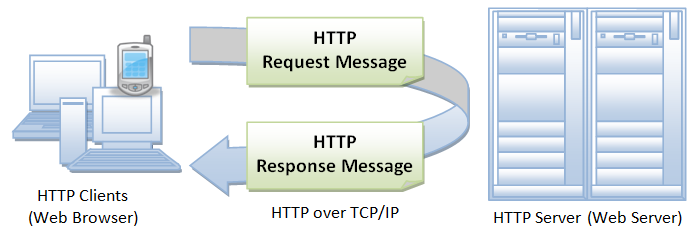
\includegraphics[width=\textwidth]{http.png}
\caption{HyperText Transfer Protocol}
\end{figure}

\section{Methodology}

\subsection{Server}
In the server side when we turn it on it will wait for any HTTP request. If it
gets any request then it will establish a connection.

After setting up the connection, it receives an http query corresponding to which file client requested. Then it will
read bytes from that file and send it to the client.

\subsection{Client}
Here our client side is any web browser. We will enter IP address of our server and the port number. Then an HTTP request will be sent from our browser to the server. 

We will see links to some files that the server provided. If we click any of them we can download them in our pc.

\section{Experimental result}

Some Snapshots of the Client Side queries can be seen in the following figures: 
\begin{figure}[!h]
\centering
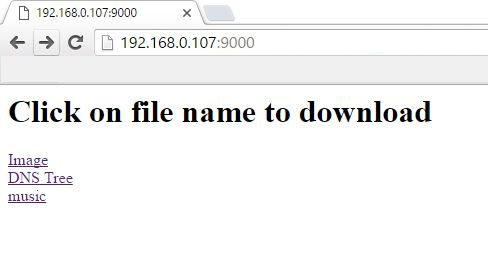
\includegraphics[width=\textwidth]{Request.JPG}
\caption{Content of Server}
\end{figure}

\begin{figure}[!h]
\centering
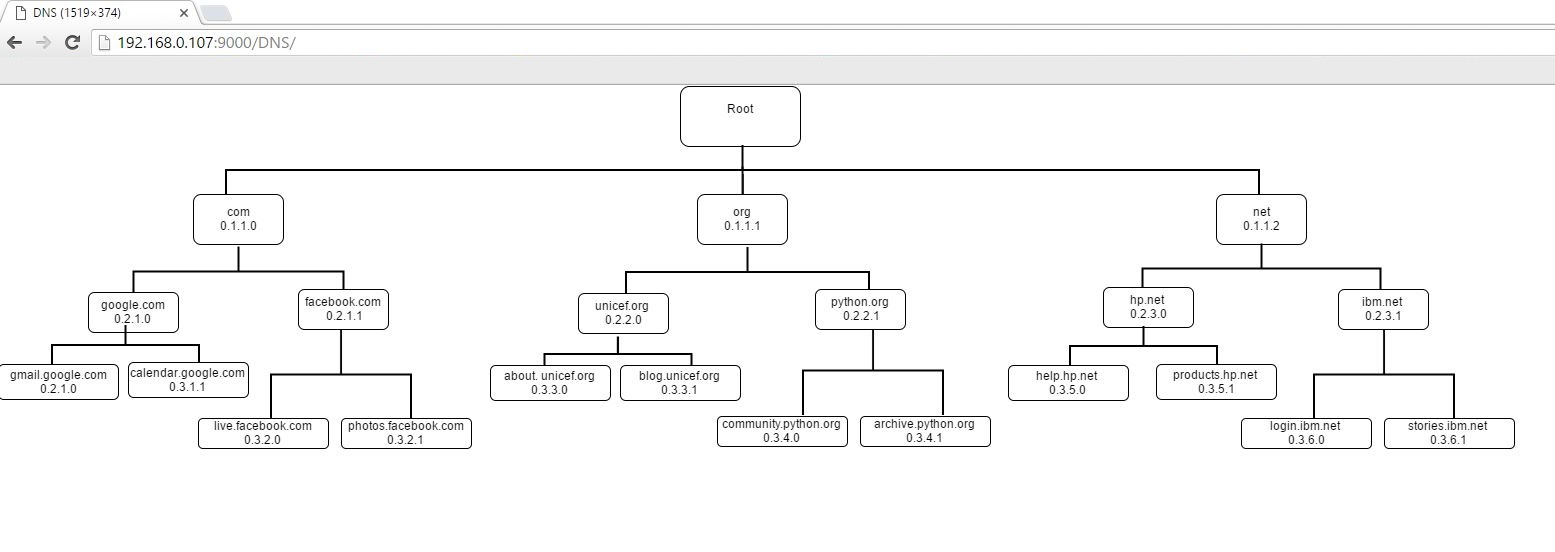
\includegraphics[width=\textwidth]{Result.JPG}
\caption{Client Side View after successful request}
\end{figure}


\newpage
\section{Experience}
\begin{enumerate}
\item We had to see some examples of how to use HttpServer package in Java
\item We used html tags for the first time to create the links.
\end{enumerate}

\begin{thebibliography}{1}
\bibitem{book}  Computer networking : a top-down approach 6th ed.
\bibitem{StackOverflow} StackOverflow : \url{http://stackoverflow.com/}
\bibitem{W3School} HTML Codes : \url{http://www.w3schools.com/}
\end{thebibliography}

\end{document}